\chapter{Diseño e implementación} % Main chapter title

\label{Chapter3} % Change X to a consecutive number; for referencing this chapter elsewhere, use \ref{ChapterX}

Este capítulo presenta la solución desarrollada para abordar el análisis multitemporal de la ocurrencia de agua en el Salar de Llullaillaco. Se describen la arquitectura general del sistema, el preprocesamiento aplicado a las imágenes satelitales, el tratamiento de datos climáticos y espectrales, el análisis temporal y la correlación con los indicadores del fenómeno ENSO. 


\definecolor{mygreen}{rgb}{0,0.6,0}
\definecolor{mygray}{rgb}{0.5,0.5,0.5}
\definecolor{mymauve}{rgb}{0.58,0,0.82}

%%%%%%%%%%%%%%%%%%%%%%%%%%%%%%%%%%%%%%%%%%%%%%%%%%%%%%%%%%%%%%%%%%%%%%%%%%%%%
% parámetros para configurar el formato del código en los entornos lstlisting
%%%%%%%%%%%%%%%%%%%%%%%%%%%%%%%%%%%%%%%%%%%%%%%%%%%%%%%%%%%%%%%%%%%%%%%%%%%%%
\lstset{ %
  backgroundcolor=\color{white},   % choose the background color; you must add \usepackage{color} or \usepackage{xcolor}
  basicstyle=\footnotesize,        % the size of the fonts that are used for the code
  breakatwhitespace=false,         % sets if automatic breaks should only happen at whitespace
  breaklines=true,                 % sets automatic line breaking
  captionpos=b,                    % sets the caption-position to bottom
  commentstyle=\color{mygreen},    % comment style
  deletekeywords={...},            % if you want to delete keywords from the given language
  %escapeinside={\%*}{*)},          % if you want to add LaTeX within your code
  %extendedchars=true,              % lets you use non-ASCII characters; for 8-bits encodings only, does not work with UTF-8
  %frame=single,	                % adds a frame around the code
  keepspaces=true,                 % keeps spaces in text, useful for keeping indentation of code (possibly needs columns=flexible)
  keywordstyle=\color{blue},       % keyword style
  language=[ANSI]C,                % the language of the code
  %otherkeywords={*,...},           % if you want to add more keywords to the set
  numbers=left,                    % where to put the line-numbers; possible values are (none, left, right)
  numbersep=5pt,                   % how far the line-numbers are from the code
  numberstyle=\tiny\color{mygray}, % the style that is used for the line-numbers
  rulecolor=\color{black},         % if not set, the frame-color may be changed on line-breaks within not-black text (e.g. comments (green here))
  showspaces=false,                % show spaces everywhere adding particular underscores; it overrides 'showstringspaces'
  showstringspaces=false,          % underline spaces within strings only
  showtabs=false,                  % show tabs within strings adding particular underscores
  stepnumber=1,                    % the step between two line-numbers. If it's 1, each line will be numbered
  stringstyle=\color{mymauve},     % string literal style
  tabsize=2,	                   % sets default tabsize to 2 spaces
  title=\lstname,                  % show the filename of files included with \lstinputlisting; also try caption instead of title
  morecomment=[s]{/*}{*/}
}


%----------------------------------------------------------------------------------------
%	SECTION 1
%----------------------------------------------------------------------------------------

\section{Área de estudio y representación espacial}

La cuenca hidrográfica del  Salar de Llullaillaco incluye sectores volcánicos elevados y drenajes que desembocan sobre el salar lo que genera condiciones potenciales para la ocurrencia de cuerpos de agua temporales. Esta delimitación hidrológica se muestra en la figura~\ref{fig:cuenca_llullaillaco}.


\begin{figure}[htpb]
	\centering
	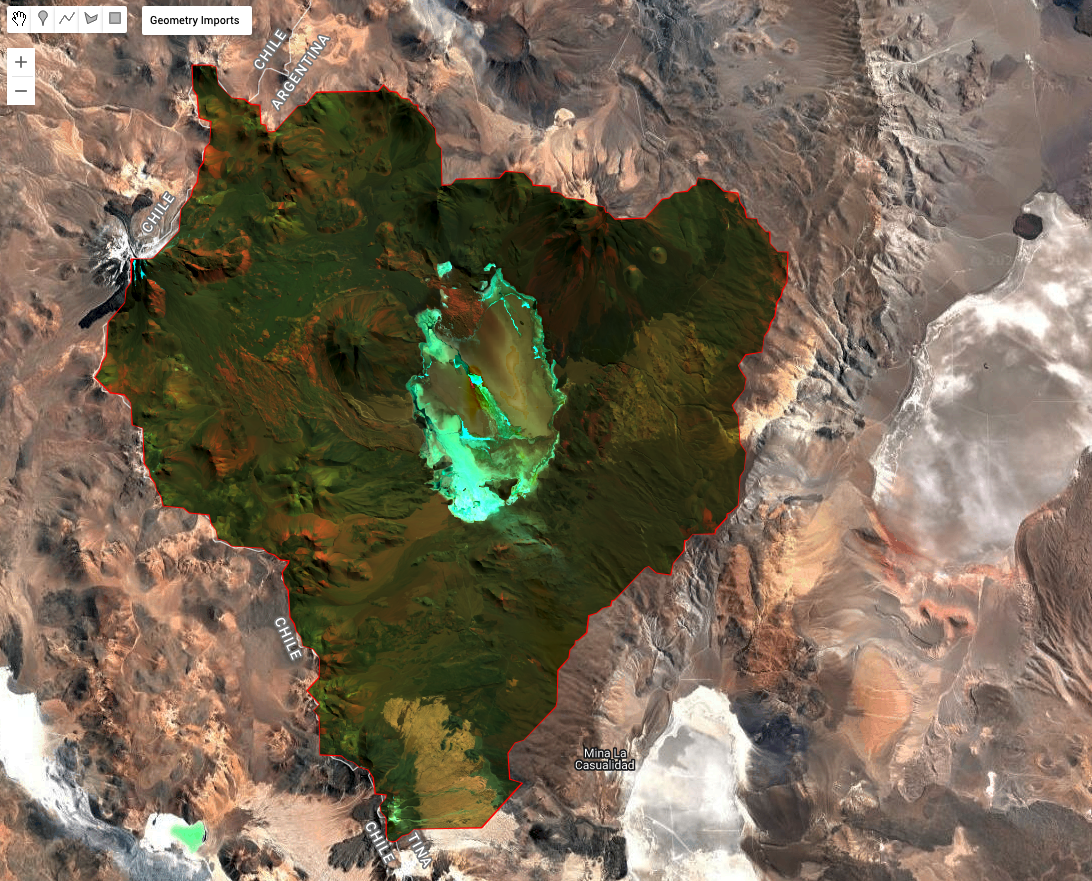
\includegraphics[scale=.3]{Figures/fig5.png}
	\caption{Cuenca del Salar de Llullaillaco.}
	\label{fig:cuenca_llullaillaco}
\end{figure}

Para determinar las zonas con mayor recurrencia de agua superficial, se implementó un procedimiento de clasificación píxel a píxel basado en la aplicación de un umbral de NDWI $>0{,}15$ sobre cada imagen mensual. Este proceso permitió generar una máscara binaria de agua para cada imagen que se integró posteriormente en un mapa de calor de ocurrencia. La proporción de imágenes en las que un píxel fue clasificado como \texttt{agua} se interpreta como una probabilidad relativa de presencia hídrica.

El resultado de este análisis se presenta en la figura~\ref{fig:mapa_ocurrencias}, donde se observan claramente las zonas de mayor persistencia de agua dentro del salar.


\begin{figure}[htpb]
	\centering
	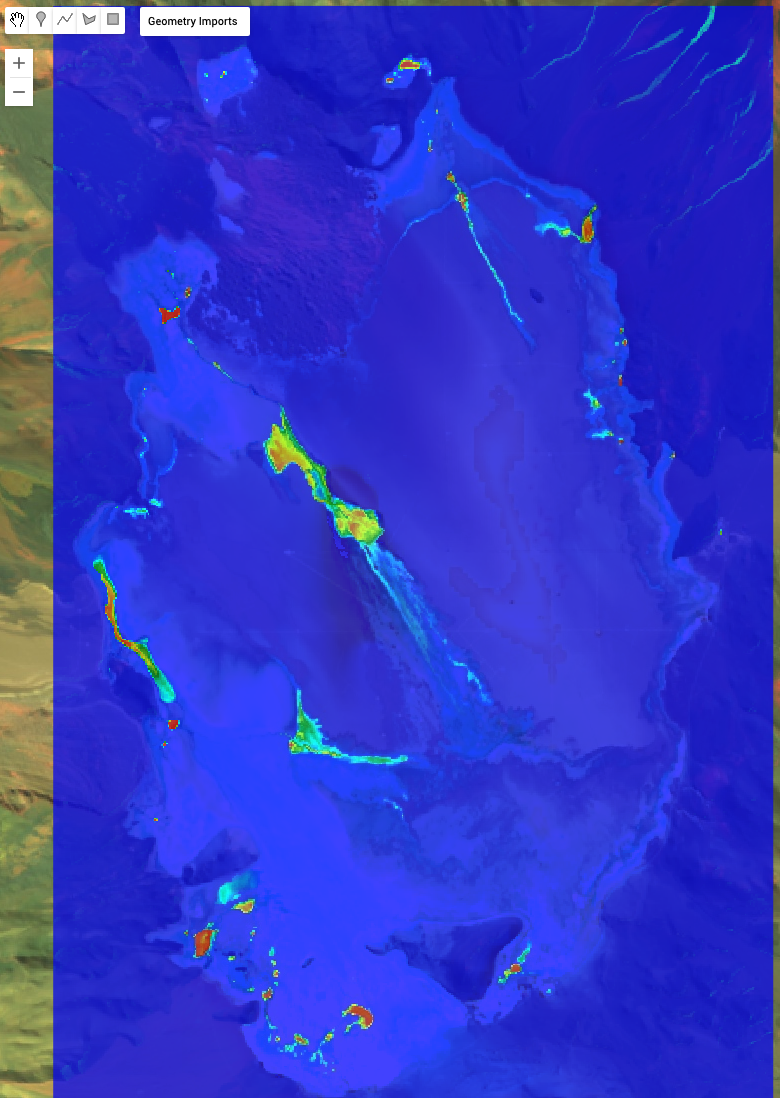
\includegraphics[scale=.3]{Figures/fig6.png}
	\caption{Mapa de calor de ocurrencia de agua superficial en el Salar de Llullaillaco. Colores más cálidos indican mayor frecuencia.}
	\label{fig:mapa_ocurrencias}
\end{figure}



\subsection{Recorte geográfico y generación de mosaicos}

La zona de estudio fue definida a partir de un polígono de delimitación del Salar de Llullaillaco, construido con herramientas SIG y validado mediante visualización satelital. A cada imagen Landsat filtrada se le aplicó un recorte espacial que limita el análisis exclusivamente a esta región.

Dado que cada misión Landsat posee distinto patrón de cobertura espacial y que algunas escenas individuales no cubren completamente el salar, se generaron mosaicos mensuales por misión donde se usó la mediana de los valores de reflectancia en cada píxel. Este procedimiento homogeniza la observación mensual y permite una mejor comparación interanual.


Se observa que la zona con mayor recurrencia de agua corresponde a la laguna central del salar, un cuerpo de agua de morfología alargada, ubicado en el eje norte-sur de la depresión principal. Por este motivo, el análisis estadístico y la posterior implementación de modelos predictivos se enfocan principalmente en esa área. Desde el punto de vista de la biodiversidad esta laguna es la que presenta mayor concentración de fauna acuática.

La figura~\ref{fig:epoca_seca_hum}  permiten visualizar el cambio estacional en la extensión de la laguna central del Salar de Llullaillaco y muestran diferencias notables entre los meses secos y húmedos.


\begin{figure}[ht]
        \centering
        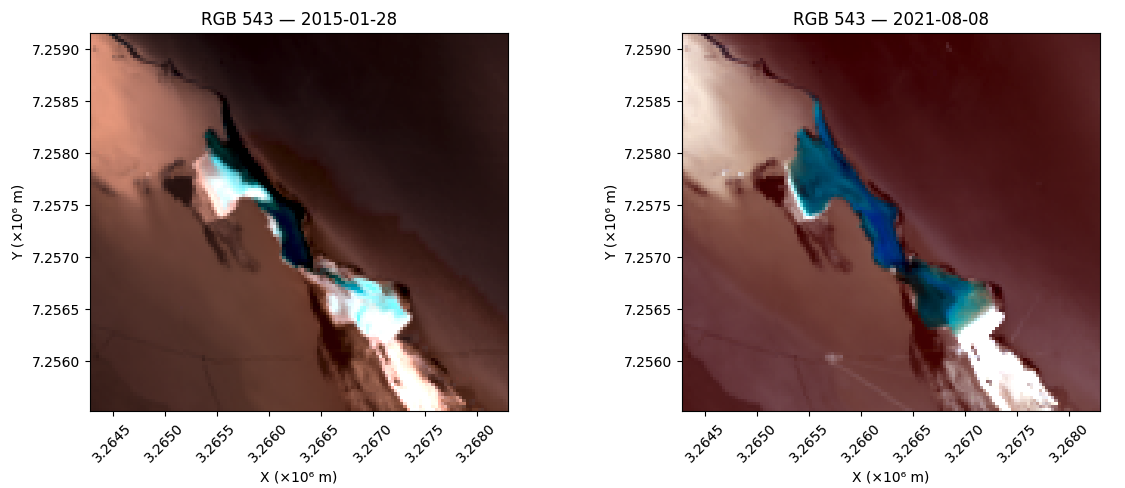
\includegraphics[scale=.37]
        {Figures/rbg_cap3_a.png}
        \caption{Imagen en composición RGB 543. Izquierda: época seca (enero 2015). Derecha: época húmeda (agosto 2021).}
        \label{fig:epoca_seca_hum}
\end{figure}


La figura~\ref{fig:ndwi_seco_hum} muestra el índice NDWI para dos fechas representativas. Valores positivos de NDWI indican presencia de agua.


\begin{figure}[ht]
        \centering
        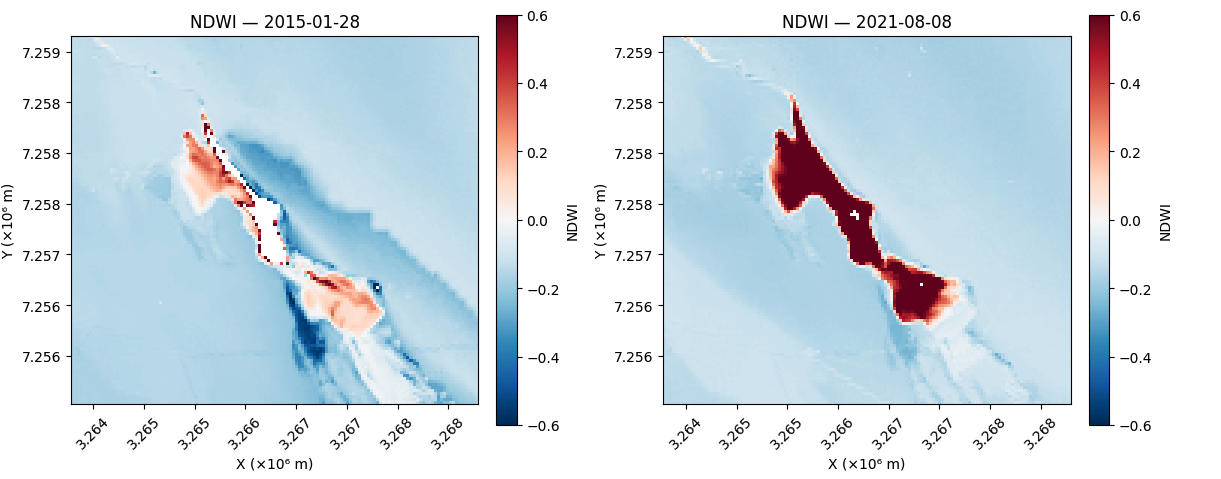
\includegraphics[scale=.37]
        {Figures/rgb_cap3_b.png}
        \caption{Indice NDWI. Izquierda: época seca (enero 2015). Derecha: época húmeda (agosto 2021).}
        \label{fig:ndwi_seco_hum}
\end{figure}


\newpage
\section{Arquitectura general del sistema}

El sistema propuesto se basa en una arquitectura modular que integra tecnologías de teledetección, análisis de datos climáticos y modelado basado en inteligencia artificial. Esta integración permite automatizar el proceso de detección de agua superficial en el Salar de Llullaillaco y explorar su posible relación con variables climáticas globales como las asociadas al fenómeno ENSO.

\subsection*{Componentes principales}

La arquitectura general del sistema se compone de tres bloques funcionales principales (ver figura \ref{fig:arquitectura_general}):

\subsection*{Componentes principales}

La arquitectura general del sistema se compone de cuatro bloques funcionales principales (ver figura \ref{fig:arquitectura_general}):

\begin{enumerate}
    \item Bloque de adquisición y preprocesamiento: se encarga de la descarga, filtrado y procesamiento de imágenes satelitales Landsat desde la plataforma GEE. En esta etapa se recorta el área de interés, se eliminan imágenes con cobertura nubosa o mala calidad y se construye un cubo temporal mensual de reflectancias. Los vacíos se completan mediante imputación, garantizando series continuas.

    \item Bloque de segmentación automática: sobre el cubo mensual se aplicó un modelo de segmentación U-Net \citep{ronneberger2015unet}, entrenado con el esquema \textit{student–teacher} \citep{hinton2015distilling}. Para ello se seleccionó un subconjunto de imágenes, se calculó NDWI y se binarizó con un umbral de 0.15, generando las etiquetas de entrenamiento. De este modo se evitó el etiquetado manual y se logró clasificar agua/no-agua en todas las imágenes mensuales.

    \item Bloque de integración climática: incorpora las series mensuales de los indicadores ENSO (Niño 3.4, SOI y MEI), obtenidas de fuentes oficiales (NOAA, BOM, PSL), alineadas temporalmente con las series de agua derivadas de las imágenes.

    \item Bloque de análisis y modelado: a partir de las series continuas de agua y ENSO se realizaron pruebas de estacionariedad (ADF, KPSS, PP), funciones de autocorrelación (ACF, PACF) y el ajuste de modelos SARIMA y VAR. Se evaluó su capacidad predictiva mediante métricas de error (RMSE, MAE) y se analizaron interdependencias estadísticas. La implementación y validación se realizó en Google Colab con Python, garantizando replicabilidad y visualización de resultados.
\end{enumerate}


\begin{sidewaysfigure}
	\centering
	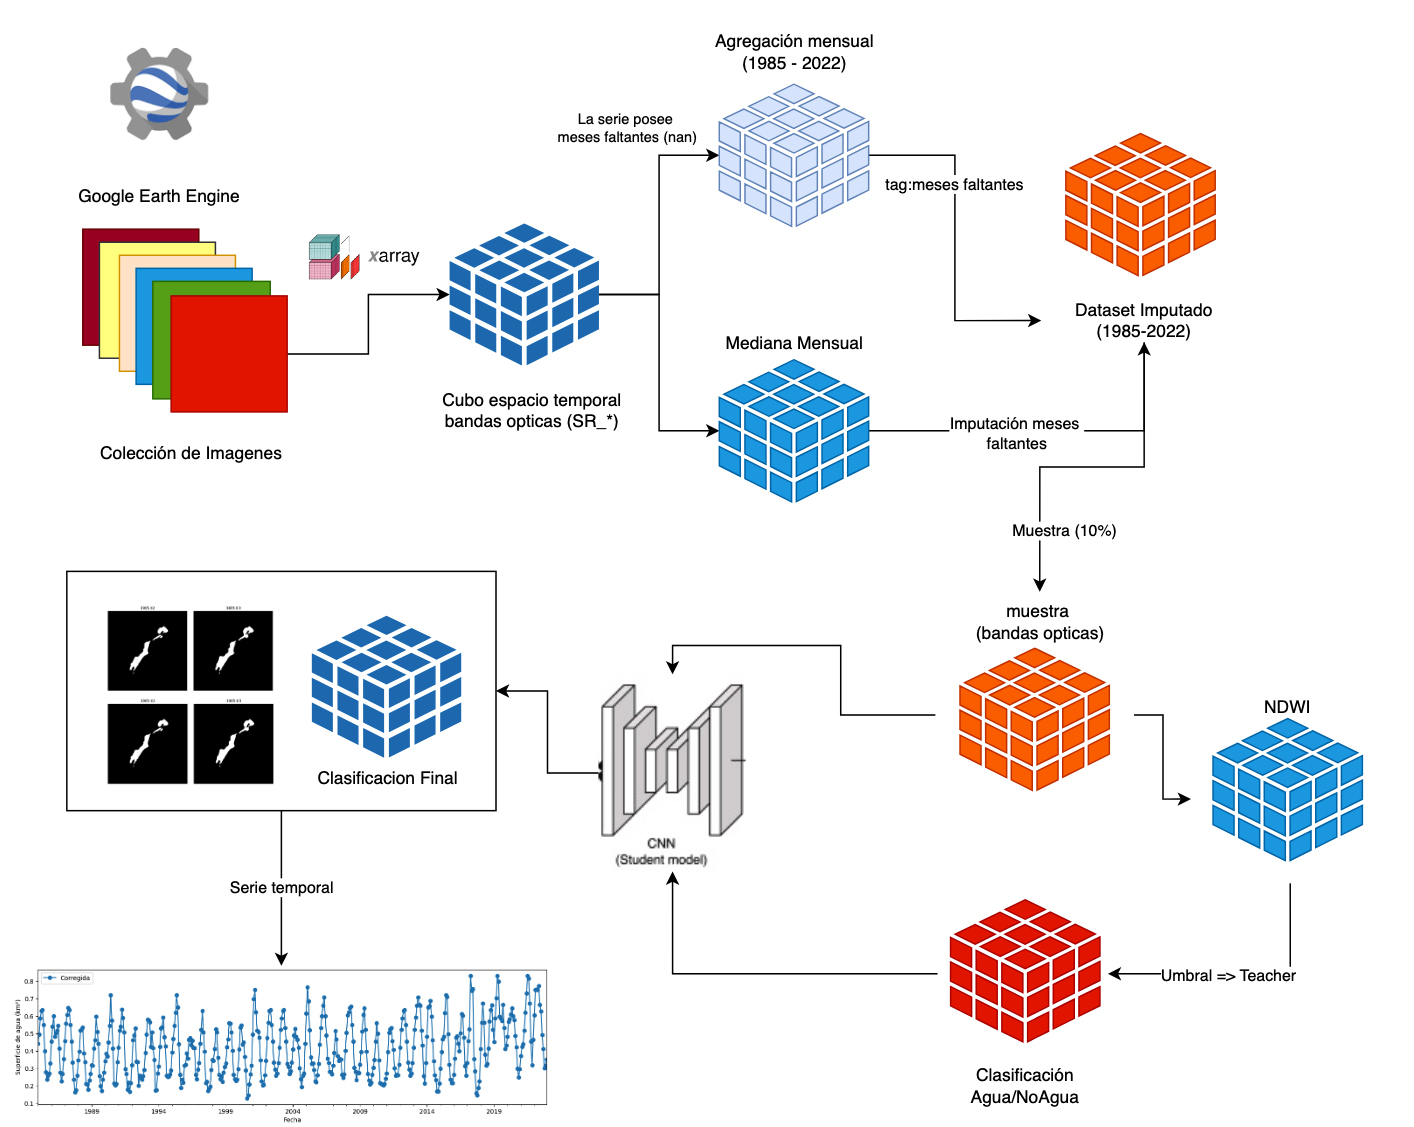
\includegraphics[scale=.4]{Figures/Arqui_TTFB22.png}
	\caption{Arquitectura general de la clasificación y generación de la serie de tiempo.}
	\label{fig:arquitectura_general}
\end{sidewaysfigure}

\begin{figure}[htpb] 
    \centering 
    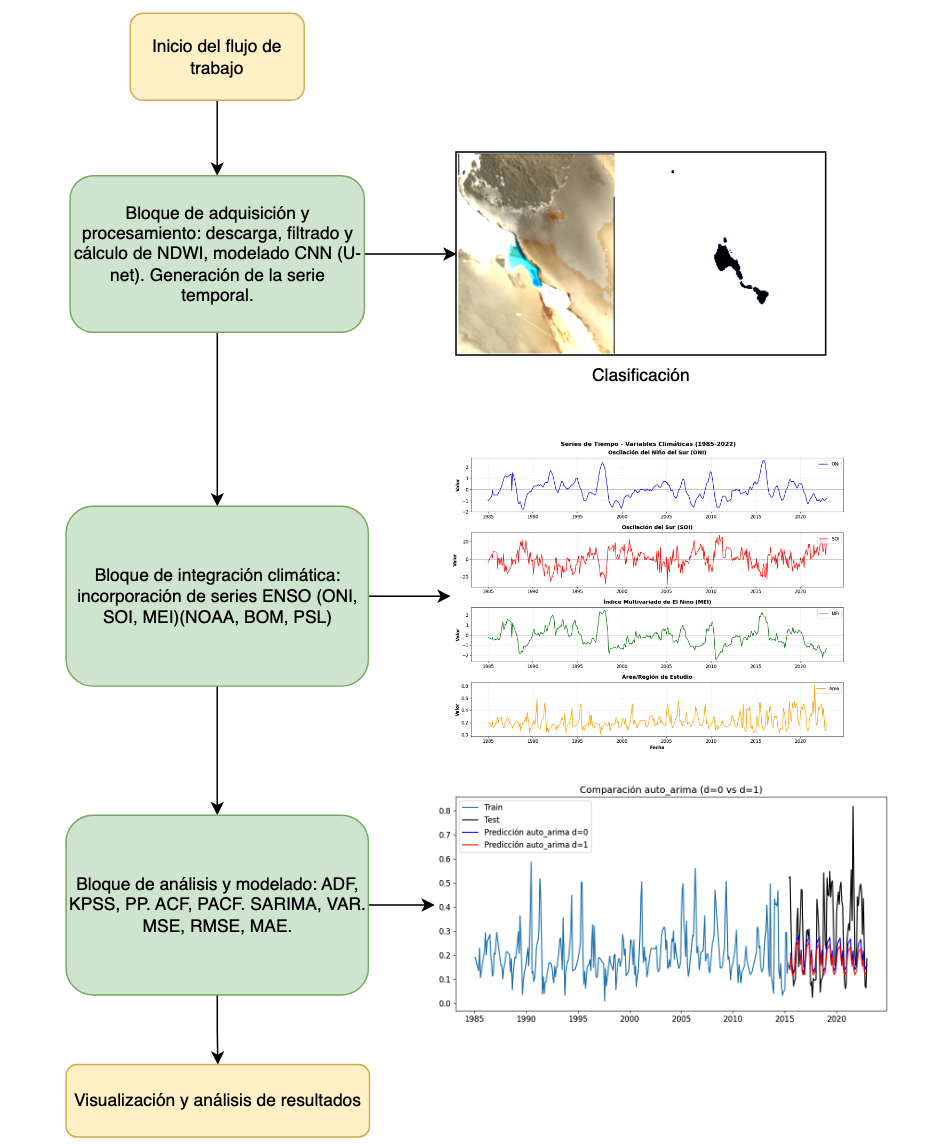
\includegraphics[scale=.4]{Figures/Arqui_TTFB3.png} 
    \caption{Arquitectura general del sistema: desde la adquisición hasta el modelado.} 
    \label{fig:arquitectura_general} 
\end{figure}

\subsection*{Flujo de trabajo detallado}

El flujo de trabajo completo incluye las siguientes etapas:

\begin{enumerate}
    \item Extracción satelital: se utilizaron las colecciones Landsat 5, Landsat 7 y Landsat 8 en GEE. Se seleccionaron imágenes con menos del 20\% de nubosidad y se recortaron al polígono del salar.

    \item Cálculo de índices: se calcularon mensualmente los valores medios de NDWI. Se generaron gráficos mensuales y una serie temporal multianual.

    \item Exportación de datos: los datos procesados en GEE fueron exportados en formato CSV y GeoTIFF para su análisis en Python.

    \item Integración con ENSO: se descargaron los valores de Niño 3.4, SOI y MEI, y se alinearon con las fechas de cada imagen mensual. Se realizaron pruebas de normalización y detección de valores atípicos.

    \item Modelado predictivo: se entrenaron modelos exploratorios para predecir la presencia/ausencia de agua en función de los índices espectrales y climáticos. Se utilizaron validaciones cruzadas y análisis de correlaciones.

    \item Visualización de resultados: se generaron mapas de ocurrencia de agua, gráficos de correlación y visualizaciones de precisión de modelos, con el objetivo de interpretar los patrones históricos y su variabilidad.
\end{enumerate}


\subsection*{Ventajas de la arquitectura}

Esta arquitectura ofrece múltiples beneficios:

\begin{itemize}
    \item Permite reproducibilidad total del flujo de trabajo mediante scripts abiertos en GEE y notebooks Python en Colab.
    \item Es escalable a otros salares o humedales de altura, con la modificación del polígono de entrada y el rango de fechas.
    \item Facilita la incorporación de nuevas fuentes climáticas o nuevos sensores remotos sin rediseñar el sistema.
    \item Optimiza el uso de recursos mediante plataformas en la nube, sin requerimientos de hardware local.
\end{itemize}

Esta solución integrada proporciona una herramienta robusta para el análisis ambiental en zonas remotas como la Puna. Su estructura modular, su compatibilidad con datos abiertos y su orientación hacia el análisis multitemporal y predictivo la convierten en una alternativa metodológica replicable en estudios de monitoreo hídrico, cambio climático y gestión territorial.


\section{Preprocesamiento de imágenes}

El preprocesamiento de imágenes satelitales constituye una etapa crítica en todo análisis multitemporal con sensores remotos. En este estudio, se utilizaron imágenes ópticas provenientes de las misiones Landsat 5 TM, Landsat 7 ETM+ y Landsat 8 OLI, accedidas desde la plataforma Google Earth Engine, que permite el procesamiento en la nube con acceso a colecciones históricas de datos corregidos radiométrica y atmosféricamente.

El objetivo del preprocesamiento fue generar series temporales limpias y comparables en el tiempo, con el fin de maximizar la calidad de los datos utilizados que son fundamentales para la detección de cuerpos de agua y vegetación residual. 

\subsubsection*{Selección y filtrado de imágenes}

Las colecciones seleccionadas corresponden a los productos nivel 2 (\texttt{L2}), que contienen valores de reflectancia de superficie corregidos atmosféricamente. Los identificadores de las colecciones utilizadas fueron:

\begin{itemize}
    \item \texttt{LANDSAT/LT05/C02/T1\_L2} para Landsat 5.
    \item \texttt{LANDSAT/LE07/C02/T1\_L2} para Landsat 7.
    \item \texttt{LANDSAT/LC08/C02/T1\_L2} para Landsat 8.
\end{itemize}

El filtrado incluyó:
\begin{itemize}
    \item Eliminación de imágenes con cobertura nubosa mayor al 20\% en la región de interés.
    \item Aplicación de máscaras QA (\textit{Quality Assessment}) para excluir píxeles cubiertos por nubes, sombras y nieve.
    \item Restricción temporal entre 1990 y 2023 y priorización de los meses húmedos (enero–abril) para asegurar observaciones relevantes.
\end{itemize}

Este filtrado permitió construir una base de imágenes consistente y sin anomalías atmosféricas notorias, adecuada para los siguientes pasos del análisis.



\subsubsection*{Corrección espectral intersensor}

Debido a diferencias en las respuestas espectrales entre las misiones (especialmente entre TM/ETM+ y OLI), se aplicó una normalización espectral basada en técnicas de remapeo lineal, tal como se propone en la literatura para combinar series temporales Landsat \parencite{roy2016characterization, roy2014landsat8}. Esto garantiza que las diferencias observadas en el índice NDWI no respondan a variaciones instrumentales sino a cambios reales en superficie.

\subsubsection*{Cálculo de índices espectrales}

Una vez preprocesadas las imágenes, se calcularon los índices espectrales mensuales para cada misión mediante el uso de las bandas adecuadas. Las bandas utilizadas para cada misión se explicaron en el capitulo anterior.

Los valores resultantes fueron exportados como series mensuales promedio para todo el salar, así como también como mapas raster por mes. Esto permitió visualizar la evolución temporal y espacial de la ocurrencia de agua superficial.

\section{Tratamiento de datos }

Esta sección presenta el tratamiento realizado sobre los datos satelitales y climáticos utilizados en el proyecto. Se detallan los criterios de selección, filtrado y preprocesamiento aplicados en la plataforma GEE, así como la integración posterior de variables climáticas globales.

\subsection*{Imágenes satelitales y período de análisis}

Se utilizaron imágenes de las misiones Landsat 5 TM, Landsat 7 ETM+ y Landsat 8 OLI, todas en su versión de corrección atmosférica de superficie (Level 2) disponible en GEE.

Para la construcción de la serie temporal se consultó las colecciones en la plataforma Google Earth Engine, correspondiente a productos de nivel 2 de Landsat 8. La selección de imágenes se restringió al polígono del Salar de Llullaillaco, al período comprendido entre 2015 y 2022, y a escenas con una cobertura nubosa menor al 20\%. Adicionalmente, se aplicó un enmascaramiento de calidad para remover nubes y sombras, con el fin de asegurar que los valores espectrales utilizados reflejaran las condiciones reales de superficie.


Si bien la misión Landsat 7 ETM+ estuvo operativa entre 1999 y 2021, su uso en este proyecto fue limitado debido a restricciones de calidad impuestas por el \textit{Scan Line Corrector (SLC)}. Este componente falló en mayo de 2003 desde donde se generaron pérdidas sistemáticas de cobertura espacial en las imágenes posteriores. Aunque en GEE existen funciones para rellenar o enmascarar los bordes afectados, se priorizó evitar la inclusión de imágenes con geometría incompleta o necesidad de interpolación espacial forzada.

La misión Landsat 5 TM fue seleccionada como fuente principal de imágenes anteriores al año 2011, ya que proporcionó datos continuos entre los años 2000 y 2011 sin fallas estructurales. Su cobertura en la región fue consistente durante la ventana húmeda seleccionada (enero a abril), con una densidad de imágenes suficiente para construir una serie temporal representativa.

Por otro lado, Landsat 8 OLI fue utilizado como principal fuente para el período comprendido entre los años 2013 y 2024. 

En la figura ~\ref{fig:cob_temporal} y en la tabla ~\ref{tab:periodos_landsat} se muestran los períodos de tiempo usados. Es necesario mencionar que debido a la superposición entre Landsat 5 TM y Landsat 7 ETM+ se decidió trabajar solo con Landsat 5 TM y Landsat 8 OLI. Se generó una brecha sin imágenes de 12 meses entre febrero de 2012 y febrero de 2013.

\begin{figure}[ht]
        \centering
        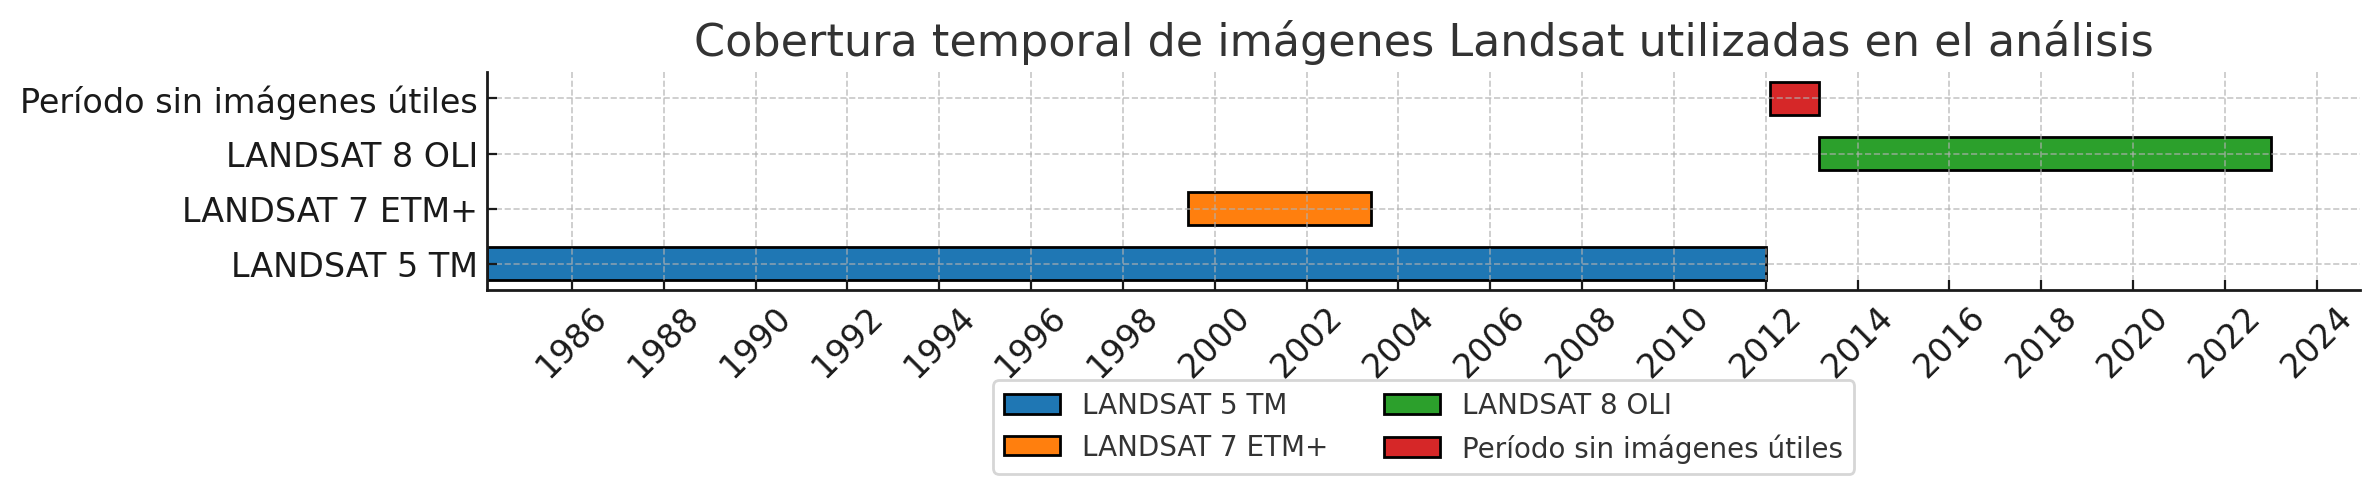
\includegraphics[scale=.4]
        {Figures/fig11.png}
        \caption{Cobertura temporal de las imágenes usadas.}
        \label{fig:cob_temporal}
\end{figure}

En resumen, la elección de misiones respondió a un compromiso entre calidad geométrica, continuidad temporal y cobertura atmosférica. Además,  se priorizó la robustez de las series en períodos relevantes para el análisis hidrológico del salar. En la figura ~\ref{fig:cant_imagenes} y en la tabla ~\ref{tab:periodos_landsat} se muestra la cantidad de imagenes usadas. 


\begin{table}[h]
	\centering
	\caption[Períodos Landsat]{Períodos de utilización de imágenes satelitales por misión Landsat en el presente estudio.}
	\begin{tabular}{l c c c}    
		\toprule
		\textbf{Misión}     & \textbf{Inicio (mes/año)} & \textbf{Fin (mes/año)} & \textbf{Cantidad de imágenes} \\
		\midrule
		Landsat 5 TM        & Marzo 1984   & Enero 2012        & 338 \\		
		Landsat 7 ETM+      & Junio 1999   & Mayo 2003         & no empleadas \\
		Landsat 8 OLI       & Marzo 2013   & Diciembre 2022    & 209 \\
		\bottomrule
	\end{tabular}
        \hline
	\label{tab:periodos_landsat}
\end{table}

\begin{figure}[ht]
        \centering
        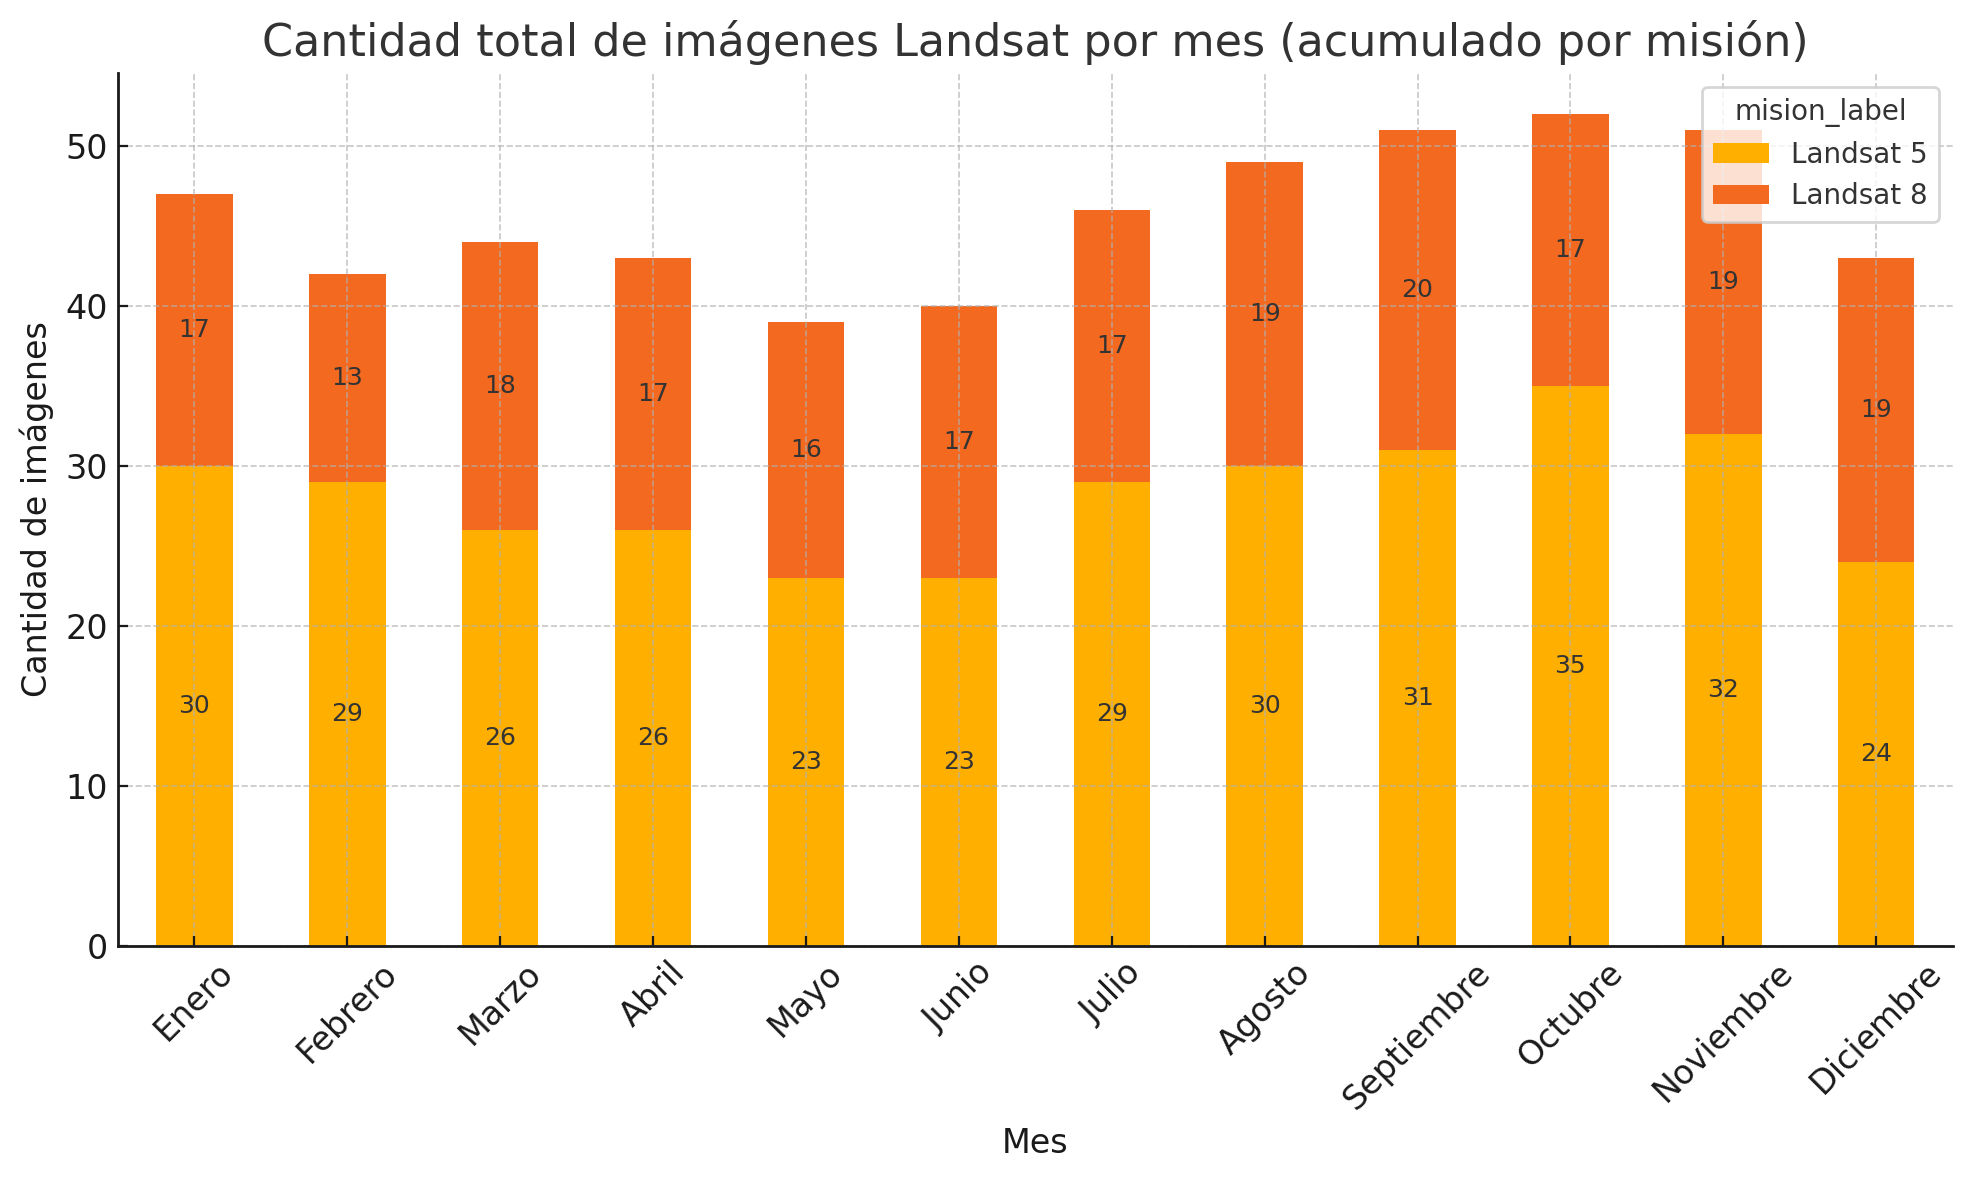
\includegraphics[scale=.4]
        {Figures/fig12.png}
        \caption{Cantidad de imágenes por mes y misión.}
        \label{fig:cant_imagenes}
\end{figure}

\subsection{Construcción del cubo temporal (xarray) desde GEE}
A partir de las consultas en Google Earth Engine (GEE), las colecciones Landsat fueron descargadas y organizadas localmente en un \emph{cubo de datos} espacio–temporal mediante \texttt{xarray}. Este cubo preserva la indexación temporal (fecha) y espacial (filas/columnas) y permite operaciones vectorizadas para apilado, reproyección y enmascaramiento de calidad. A continuación se presenta un ejemplo de 4 imágenes dentro del cubo de datos~\ref{fig:agg_mens}.

\begin{figure}[ht]
        \centering
        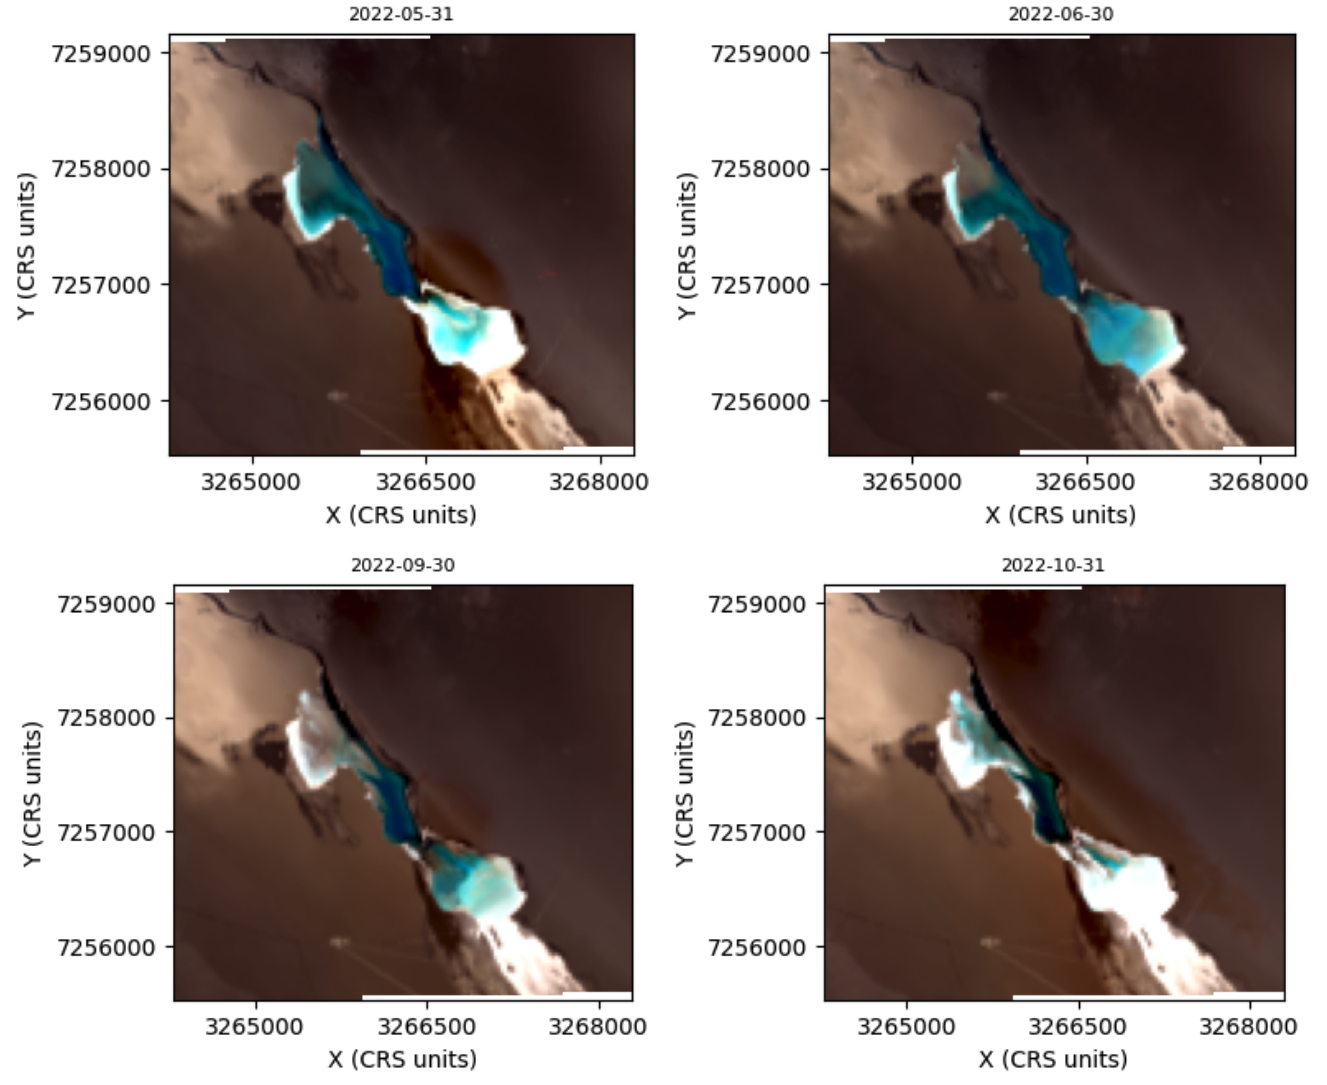
\includegraphics[scale=.25]
        {Figures/agg_mens.png}
        \caption{Imágenes de ejemplo del cubo temporal de imágenes.}
        \label{fig:agg_mens}
\end{figure}

\begin{figure}[htpb]
    \centering
    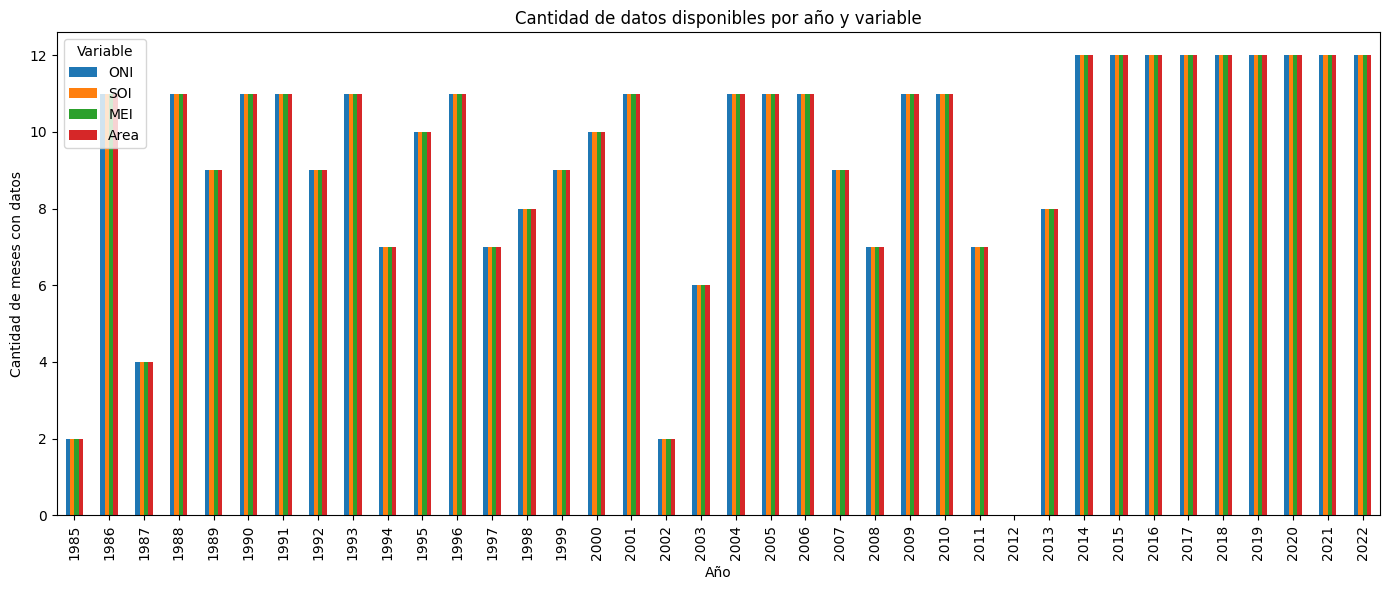
\includegraphics[scale=.40]{Figures/conteo_series.png}
    \caption{Cantidad de meses con datos disponibles por año y variable (ONI, SOI, MEI, Área).}
    \label{fig:conteo_datos}
\end{figure}

\subsection{Agregación mensual e imputación de meses faltantes}
El cubo diario de imagen inicial fue agregado a escala \emph{mensual} (mediana de reflectancia) para homogeneizar la frecuencia de análisis. Dado que algunos meses carecían de imágenes válidas(ver figura~\ref{fig:conteo_datos}, se generó un cubo mensual \emph{imputado} aplicando la estrategia de promedio mensual histórico para imágenes mensuales ausentes. El resultado es un cubo mensual continuo que sostiene las etapas posteriores de segmentación y series temporales. A continuación se presenta las imágenes mensuales (mediana) dentro del cubo de datos~\ref{fig:agg_mens}.

\begin{figure}[ht]
        \centering
        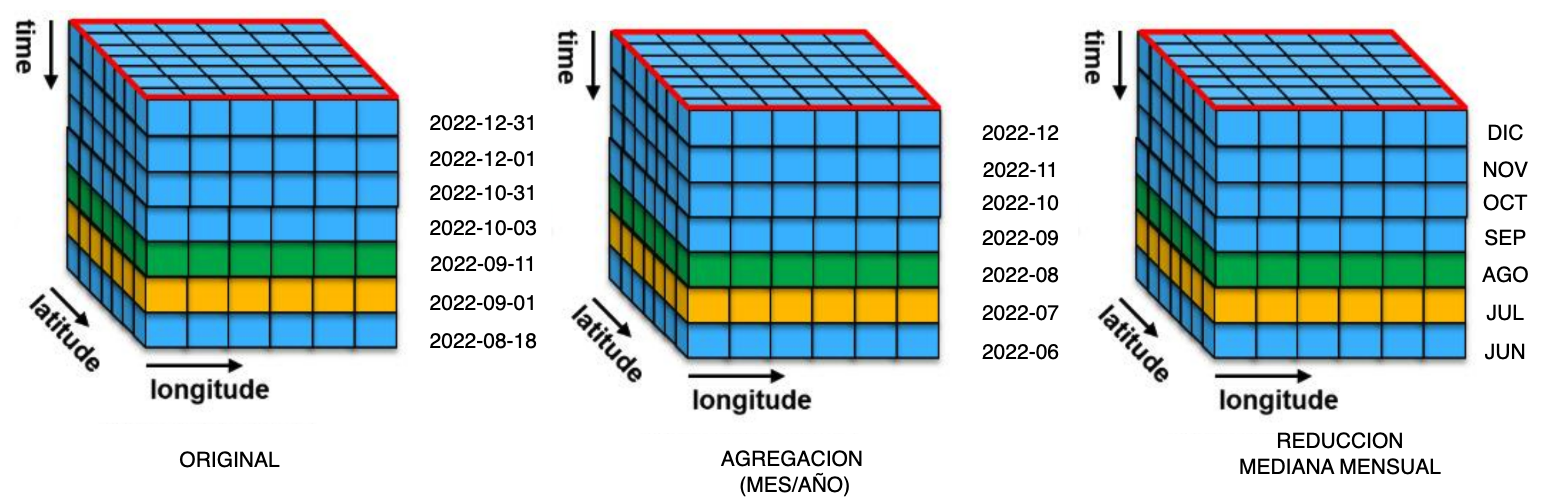
\includegraphics[scale=.25]
        {Figures/cube.png}
        \caption{Ejemplo de agregaciones y reducciones usando cubos temporales.}
        \label{fig:img_mens}
\end{figure}


\begin{figure}[ht]
        \centering
        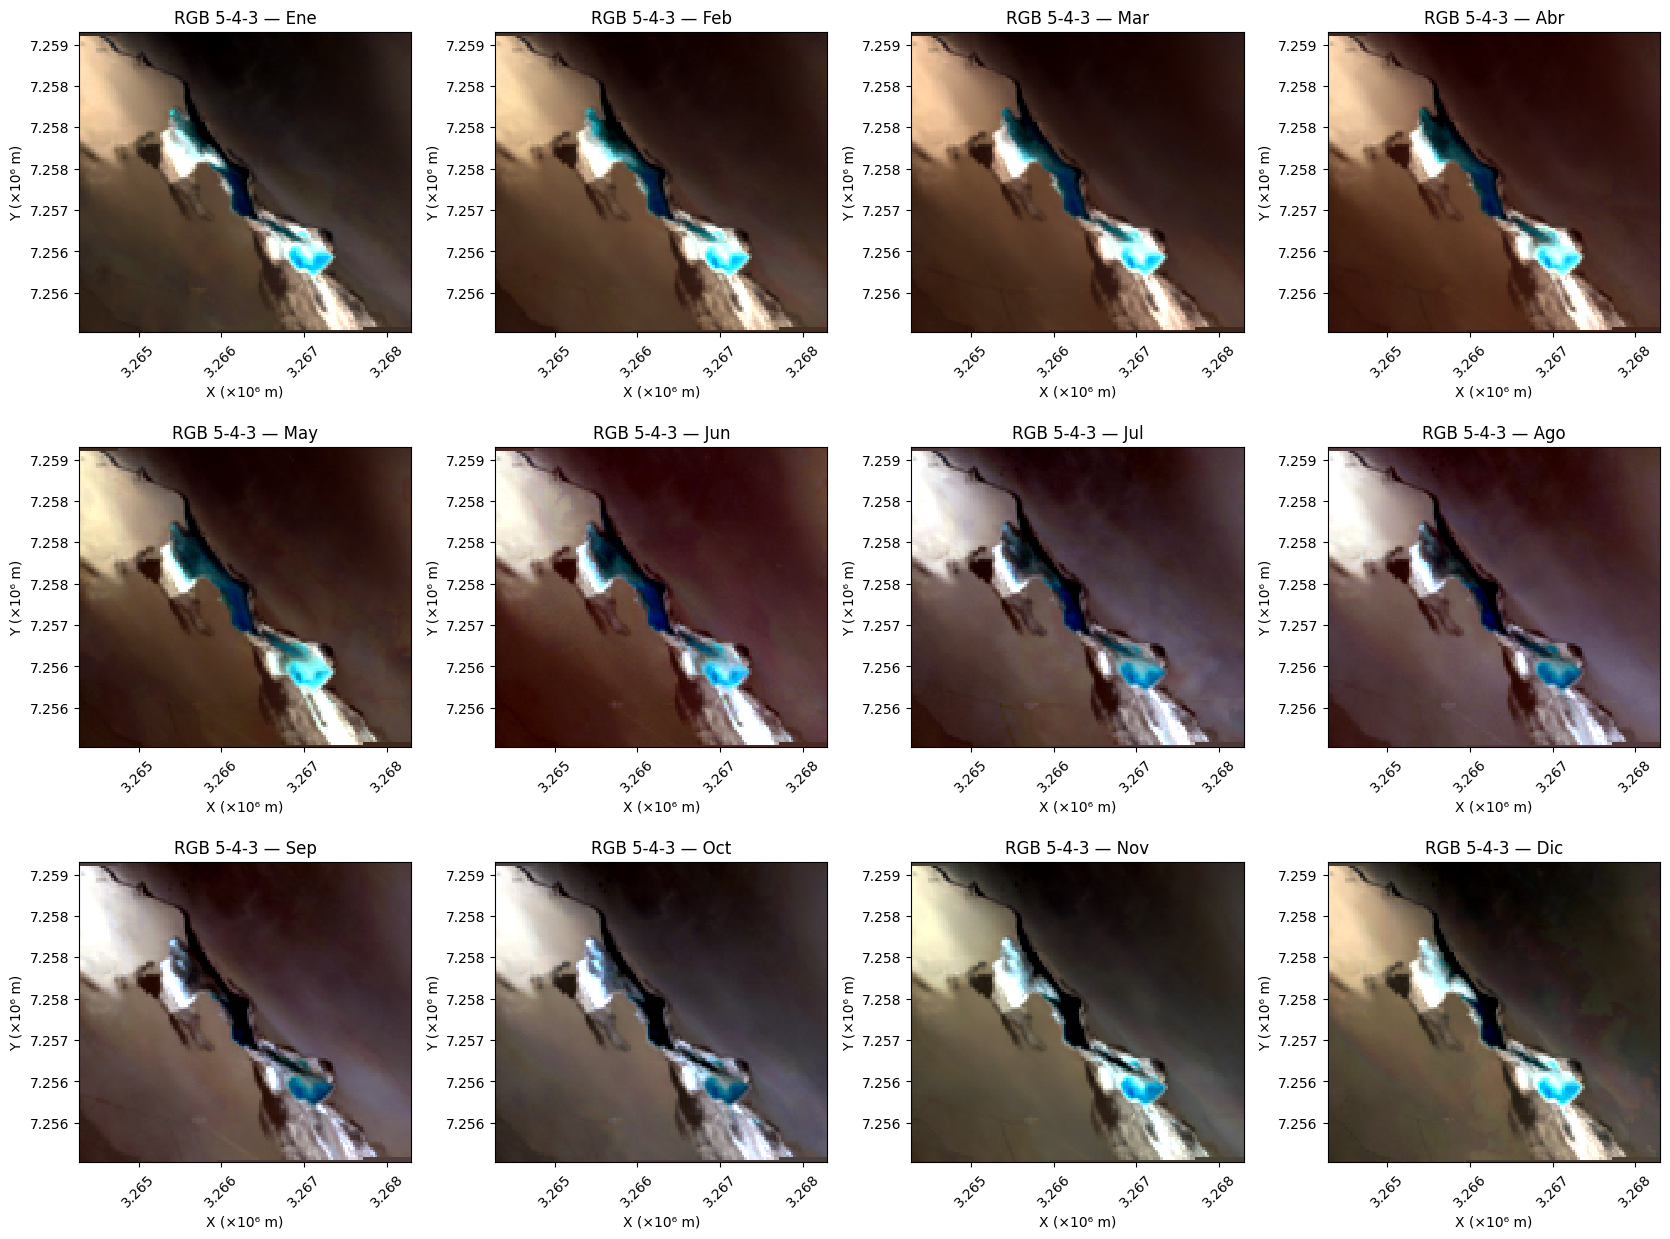
\includegraphics[scale=.30]
        {Figures/mensualimg_.png}
        \caption{Imágenes medianas mensuales de la serie histórica.}
        \label{fig:img_mens}
\end{figure}

\section{Segmentación de las imágenes}

En este trabajo se toma como referencia la metodología \emph{DeepAqua}\cite{DeepAqua2023}, que aplica arquitecturas de redes neuronales convolucionales tipo U-Net para la detección y cartografía de cuerpos de agua en imágenes satelitales. 

\begin{figure}[ht]
        \centering
        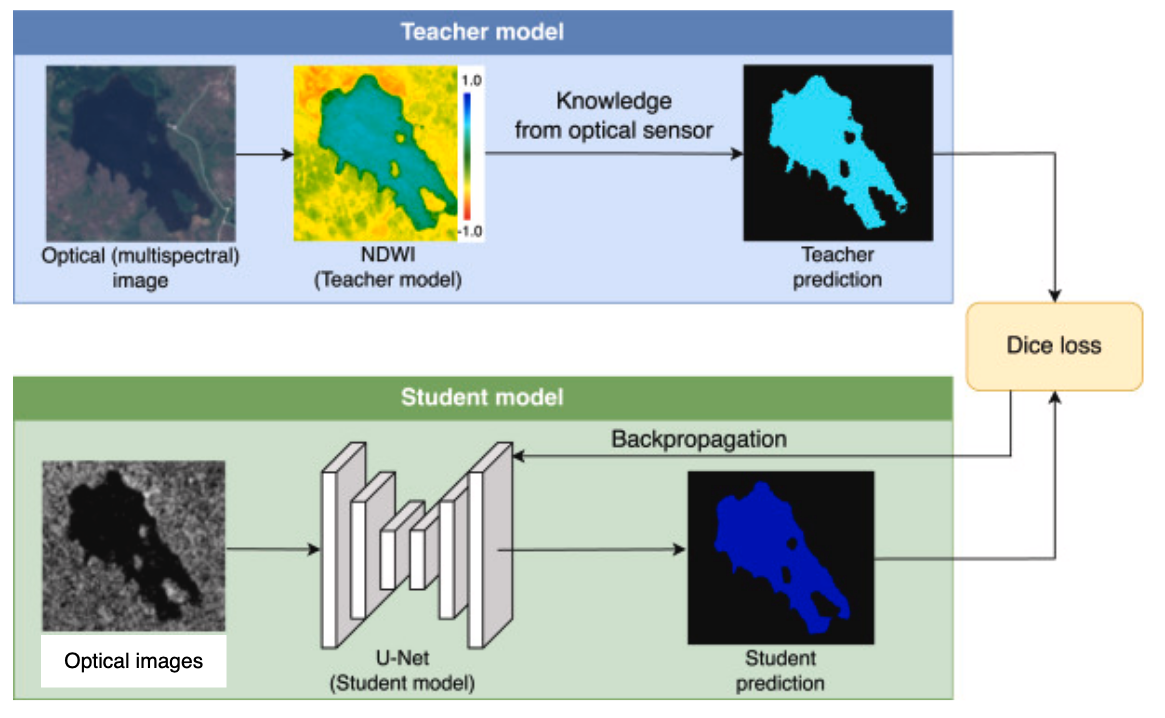
\includegraphics[scale=.20]
        {Figures/deep_2.png}
        \caption{Esquema de trabajo Teacher-Student para clasificación.}
        \label{fig:img_mens}
\end{figure}

\subsection{U-Net mediante etiquetado débil (student--teacher)}
Para evitar el etiquetado manual, se adoptó una estrategia \emph{student--teacher} (distilación de conocimiento). Se seleccionó aleatoriamente un 5\% de los meses del cubo mensual imputado; sobre ese subconjunto se calculó NDWI mensual y se aplicó un umbral \ de 0{,}15 para binarizar agua/no agua (rol \emph{teacher}). Estas máscaras sirvieron como \emph{pseudo-etiquetas} para entrenar una CNN tipo U-Net \parencite{ronneberger2015unet}, usando como entrada las bandas ópticas del mismo mes.

La U-Net (\emph{student}) aprendió un mapeo robusto a partir de pseudo-etiquetas ruidosas, aprovechando regularización espacial y multiescala propias de la arquitectura. Una vez entrenado el modelo, se segmentaron \emph{todos} los meses del cubo, reemplazando la binarización por umbral con predicciones consistentes espacial y temporalmente. Este esquema reduce sesgo por umbrales fijos y evita la dependencia de etiquetas manuales, en línea con la idea de \emph{distilación} \parencite{hinton2015distilling}. 

La arquitectura utilizada corresponde a una U-Net de pequeña escala (\textit{UNetSmall}), diseñada específicamente para tareas de segmentación binaria. El modelo se estructura en tres bloques principales:

\begin{itemize}
    \item Codificador (encoder): compuesto por tres bloques de convoluciones dobles (\textit{DoubleConv}) seguidos de operaciones de \textit{MaxPooling}, que reducen progresivamente la resolución espacial y extraen características relevantes de las imágenes de entrada.

    \item Cuello de botella (bottleneck): bloque central con convoluciones dobles, encargado de capturar representaciones de alto nivel.

    \item Decodificador (decoder): formado por capas de \texttt{ConvTranspose2d} (upsampling) y bloques \texttt{DoubleConv}, que permiten recuperar la resolución espacial original. Cada etapa del decodificador concatena las salidas correspondientes del encoder mediante skip connections, preservando información espacial fina.

    \item Capa de salida: una convolución $1 \times 1$ genera el mapa binario final, en este caso indicando presencia o ausencia de agua.
\end{itemize}

Este diseño mantiene la filosofía de la U-Net original \parencite{ronneberger2015unet}, pero adaptado a una escala reducida, lo que lo hace más eficiente para trabajar con cubos de imágenes mensuales de resolución moderada. A continuación se presenta las imágenes una imagen usada en el entrenamiendo con los pares student-teacher~\ref{fig:agg_mens}.


\begin{figure}[ht]
        \centering
        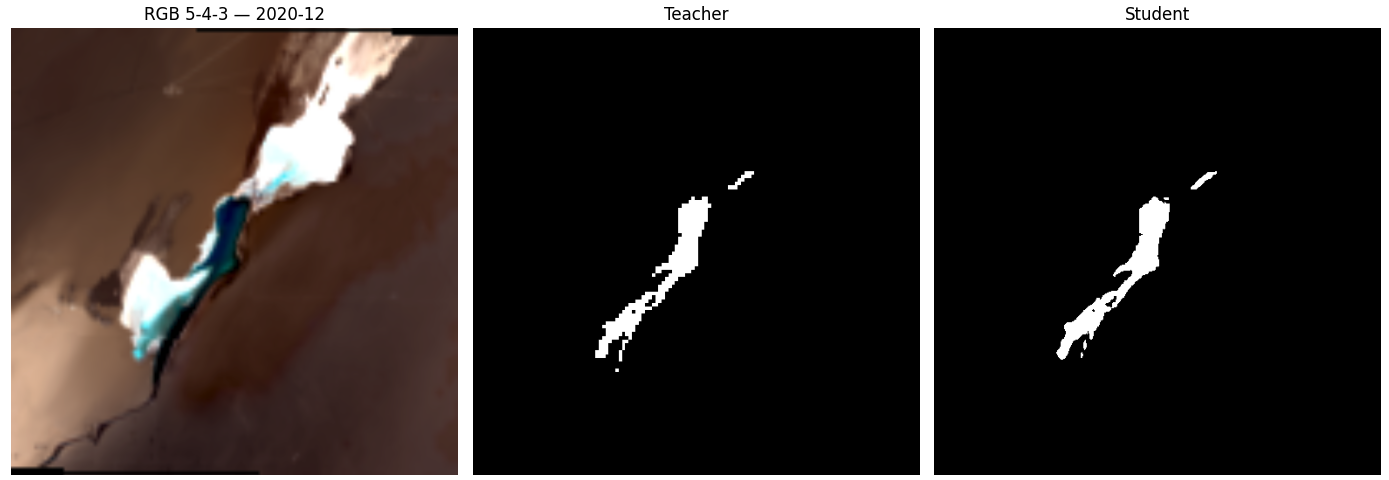
\includegraphics[scale=.25]
        {Figures/student_teacher.png}
        \caption{Resultado del esquema Teacher-Student para clasificación.}
        \label{fig:class_2}
\end{figure}



Las máscaras mensuales segmentadas por U-Net se convirtieron a área de agua por mes mediante conteo de píxeles y área efectiva de cada píxel. A continuación se presenta la serie de tiempo resultante del proceso de modelado~\ref{fig:ts_cnn}.

Esta serie mensual de \emph{Área} es la base de los análisis de series temporales y los modelos SARIMA/VAR.

\begin{figure}[ht]
        \centering
        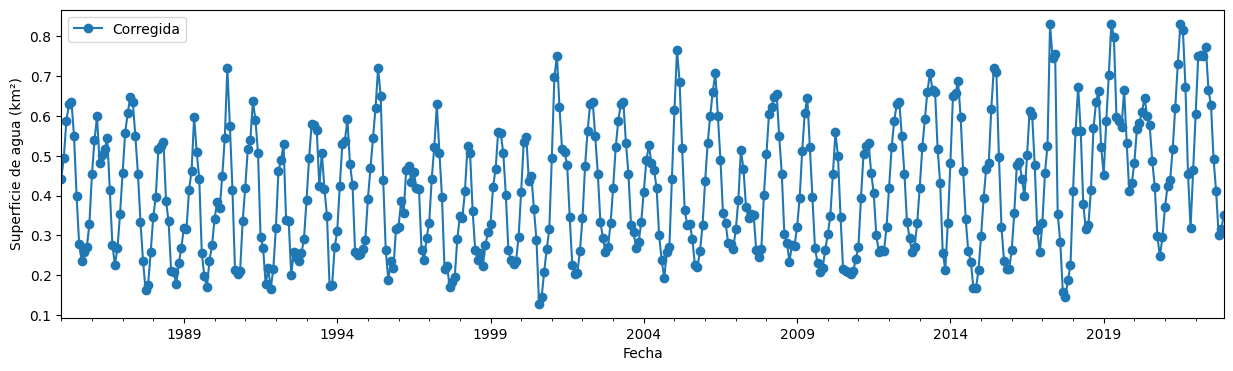
\includegraphics[scale=.45]
        {Figures/ts_final_cnn.png}
        \caption{Serie de tiempo resultante.}
        \label{fig:ts_cnn}
\end{figure}


\section{Datos climáticos globales}

Como complemento a la información satelital, se integraron series temporales mensuales de los principales índices asociados al fenómeno ENSO. Estos indicadores ya han sido presentados en el Capítulo~\ref{Chapter2}; en esta sección se detalla únicamente el tratamiento aplicado para su incorporación en el análisis.

\begin{itemize}
    \item ONI (Oceanic Niño Index): se descargaron los valores mensuales publicados por la NOAA, calculados a partir de anomalías de temperatura superficial del mar en la región Niño 3.4 \parencite{noaaONI}. La serie fue recortada al período de análisis (1984--2022) y estandarizada mediante transformación a \textit{z-score}. Los resultados se muestran en la Figura~\ref{fig:indice_oni}.
    
    \item SOI (Southern Oscillation Index): se emplearon los datos mensuales provistos por el \textit{Australian Bureau of Meteorology} \parencite{bom_soi_2024}. La serie fue ajustada para coincidir en fechas con las observaciones de agua y normalizada con \textit{z-score}. La Figura~\ref{fig:indice_soi} presenta su evolución en el período de estudio.
    
    \item MEI.v2 (Multivariate ENSO Index, versión 2): se descargaron los valores bimestrales publicados por el NOAA Physical Sciences Laboratory \parencite{meiindex}. Para este trabajo, la serie se transformó a escala mensual asignando cada valor al segundo mes del par, y posteriormente se estandarizó con \textit{z-score}. En la Figura~\ref{fig:indice_mei} se ilustra la dinámica del índice.
\end{itemize}

De esta manera, las tres series ENSO quedaron homogeneizadas en frecuencia y escala, lo que permitió su comparación directa con la serie de área de agua superficial del Salar de Llullaillaco.




\section{Series de tiempo preliminares}

Todos los índices climáticos utilizados en este estudio (ONI, SOI y MEI) fueron estandarizados mediante su transformación a \textit{z-score} para facilitar la comparación entre series con distintas escalas y unidades. En la figura~\ref{fig:indice_area} se observa la evolución temporal del área de la laguna de estudio en \textit{z-score}, mientras que en las figuras~\ref{fig:indice_oni_ts},~\ref{fig:indice_soi_ts} y~\ref{fig:indice_mei_ts} se muestran los índices ONI, SOI y MEI en \textit{z-score} respectivamente.

Se identificó que las series originales de cobertura de agua superficial y de los índices climáticos ENSO (ONI, SOI y MEI) no eran homogéneas, ya que presentaban vacíos temporales y diferencias en la disponibilidad de datos a lo largo del período de estudio. Esta heterogeneidad impedía su tratamiento directo como series de tiempo y, en consecuencia, limitaba la aplicación de algoritmos de \textit{machine learning} especializados en predicción temporal.  

Por ello, fue necesario realizar un proceso de estandarización y depuración de las series, ajustando su frecuencia y completitud para generar secuencias temporales comparables y aptas para los modelos predictivos. En la figura~\ref{fig:conteo_datos} se muestra la distribución de meses con datos disponibles por año para cada variable, lo que evidencia la falta de homogeneidad inicial. 

Posteriormente, se aplicaron técnicas de preprocesamiento y estrategias de imputación para obtener series homogéneas y continuas, que constituyen la base para el análisis de correlaciones y la construcción de modelos predictivos basados en series temporales.  

En la figura ~\ref{fig:ts_final} se muestran las series temporales resultantes.


\begin{figure}[ht]
        \centering
        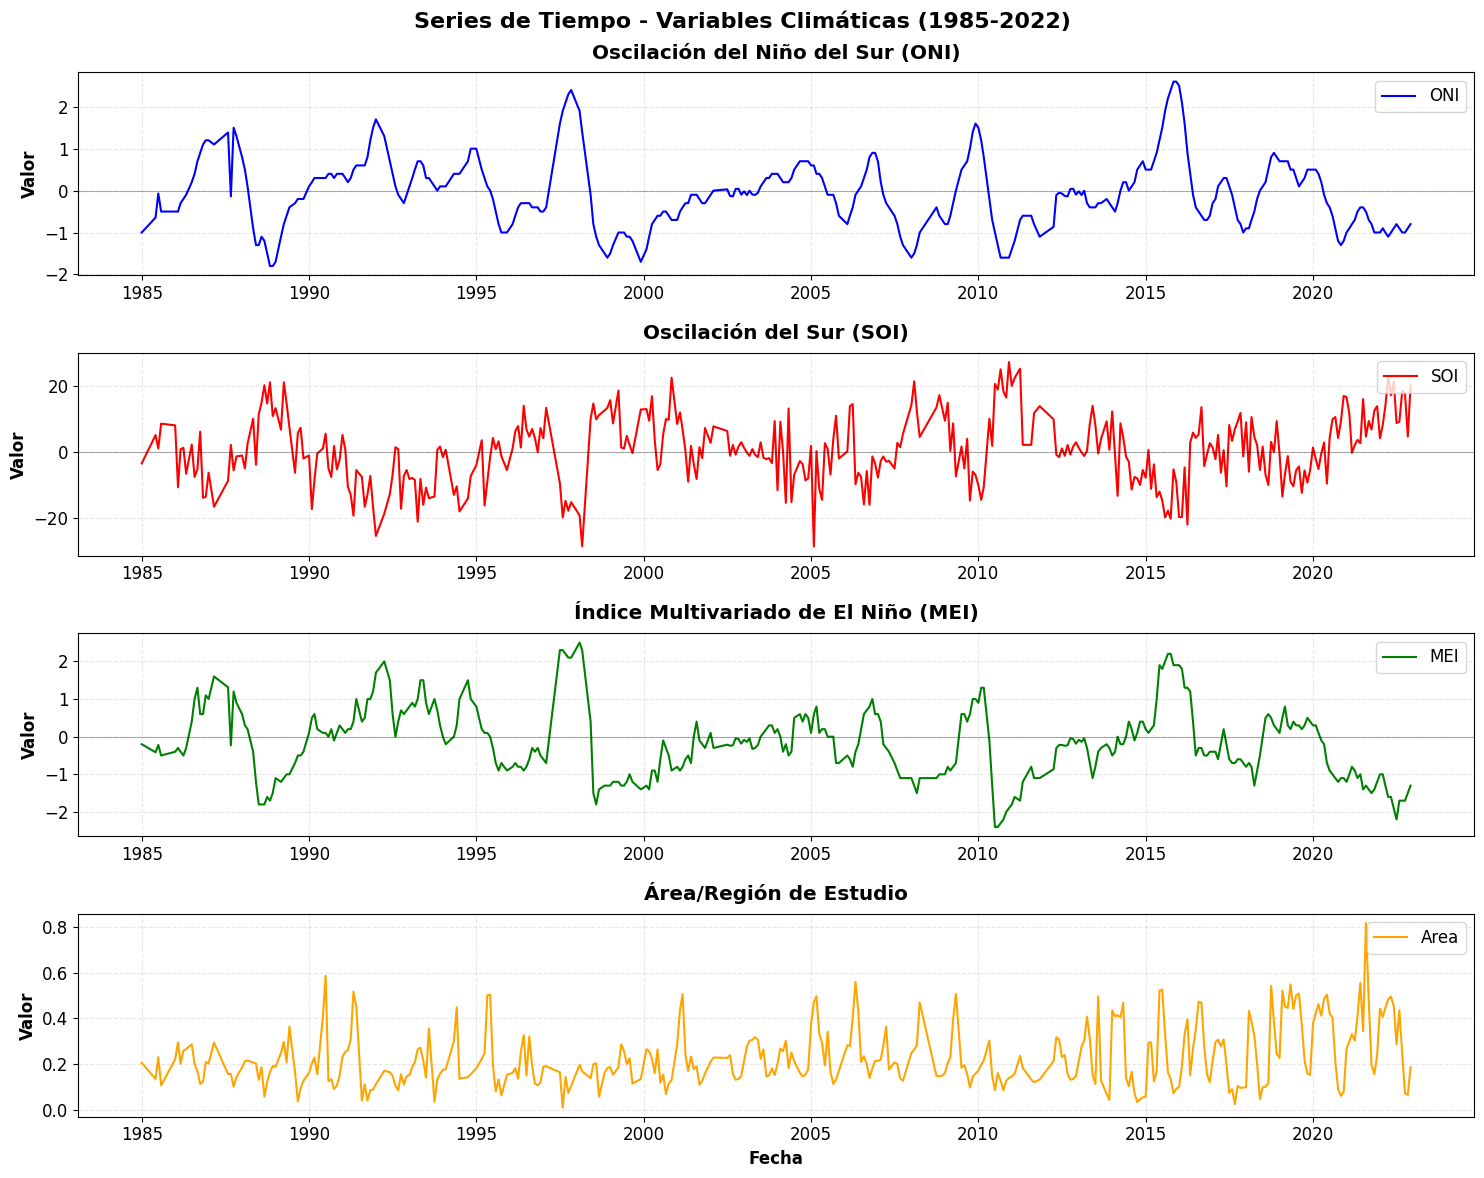
\includegraphics[scale=.32]
        {Figures/ts_final.png}
        \caption{Series temporales procesadas.}
        \label{fig:ts_final}
\end{figure}

\section{Exploración y tratamiento de las series temporales}
En esta sección se realiza una exploración de las variables a trabajar. Además, se realizan análisis visuales y comparaciones entre las variables. 

\subsection{Raíces unitarias}

Antes de la aplicación de modelos autorregresivos, se realizó un análisis visual de las 
series para explorar posibles tendencias o comportamientos no estacionarios. De manera 
preliminar, se observaron los siguientes patrones:

\begin{itemize}
    \item Serie Área (superficie de agua): muestra una tendencia descendente a lo 
    largo del período analizado, disminuyendo de valores cercanos a 0,8 hacia 0,2. Este 
    comportamiento sugiere la presencia de una deriva temporal y, por lo tanto, 
    no estacionariedad en media.
    \item Índices ENSO (ONI, SOI, MEI): presentan un comportamiento oscilatorio 
    alrededor de cero, sin tendencia ascendente o descendente clara y con variabilidad 
    relativamente constante. Estas características son típicas de series estacionarias.
\end{itemize}

Para corroborar estas observaciones se aplicó la prueba de Dickey-Fuller aumentada (ADF), cuyo objetivo es contrastar la hipótesis nula de no estacionariedad. La hipótesis nula se rechaza si el p-valor es menor a 0,05 o si el estadístico ADF es menor al valor crítico al 5\%. Los resultados obtenidos se presentan en la tabla~\ref{tab:adf_test}.

\begin{table}[H]
    \centering
    \caption{Resultados del test Dickey-Fuller aumentado (ADF)}.
    \label{tab:adf_test}
    \begin{tabular}{lccc}
        \toprule
        \textbf{Serie} & \textbf{Estadístico ADF} & \textbf{p-valor} & \textbf{Conclusión} \\
        \midrule
        ONI  & -6,5601 & 0,000000 & Estacionaria \\
        SOI  & -5,2308 & 0,000008 & Estacionaria \\
        MEI  & -5,2128 & 0,000008 & Estacionaria \\
        Área & -2,8901 & 0,046511 & Estacionaria (débil) \\
        \bottomrule
    \end{tabular}
\end{table}

Según los tests realizados es posible interpretar lo siguiente:   
\begin{itemize}
    \item ONI, SOI y MEI: resultaron fuertemente estacionarios, con p-valores 
    iguales a 0.000008 y estadísticos ADF muy por debajo de los valores críticos al 1\%. 
    Esto confirma su patrón oscilatorio estable alrededor de cero.
    \item Área: se ubicó en el límite de la estacionariedad, con un p-valor de 
    0,0465 y un estadístico ADF menor al valor crítico al 5\% pero no al 1\%. Aunque el 
    test formalmente indica estacionariedad, la tendencia descendente observada en la 
    inspección visual sugiere precaución, recomendándose aplicar diferenciación en los 
    modelos para obtener mayor robustez.
\end{itemize}


En síntesis, las series climáticas ONI, SOI y MEI no requieren diferenciación, mientras que 
la serie de Área, aunque marginalmente estacionaria según ADF, podría beneficiarse de 
una transformación adicional.

\subsection{Análisis visual de ACF y PACF}

Con el fin de explorar la estructura de dependencia temporal de cada serie, se graficaron 
las funciones de autocorrelación (ACF) y autocorrelación parcial (PACF). Estas funciones 
permiten identificar patrones de memoria temporal, evaluar la estacionariedad y orientar 
la selección de órdenes iniciales para modelos ARIMA o SARIMA \parencite{box2015time, hyndman2018forecasting}. 

\subsubsection{Variable ONI}

La ACF del ONI(~\ref{fig:facp_oni}) muestra un decaimiento lento y oscilatorio, típico de procesos con memoria 
larga y comportamiento cíclico (El Niño / La Niña). La PACF evidencia un corte abrupto 
tras los primeros rezagos (lag 1 o 2), lo que sugiere que un modelo autorregresivo de bajo 
orden (AR(1) o AR(2)) podría capturar adecuadamente su estructura.

\subsubsection{Variable SOI}

La ACF del SOI(~\ref{fig:facp_soi}) presenta un patrón de decaimiento oscilatorio persistente, con memoria de 
largo plazo. La PACF muestra un corte tras los primeros rezagos (lag 1–2), indicando que 
un modelo AR(2) constituye un buen punto de partida para esta serie.

\subsubsection{Variable MEI}

El MEI exhibe un patrón similar al ONI y SOI: la ACF(~\ref{fig:facp_mei}) decae lentamente con oscilaciones, 
mientras que la PACF se corta tras los primeros rezagos. Esto indica la presencia de 
dependencia temporal y ciclos ENSO, siendo un modelo AR(1)–AR(2) adecuado como 
aproximación inicial.

\subsubsection{Variable Área}

La ACF del Área (~\ref{fig:facp_area}) muestra un decaimiento muy lento y persistente, lo que refleja la 
presencia de una tendencia dominante y sugiere no estacionariedad. La PACF presenta un 
corte marcado en el lag 1, reforzando la necesidad de diferenciar la serie (I=1) antes de 
ajustar un modelo ARIMA. Tras la diferenciación, un modelo AR(1) constituye un punto de 
partida razonable.

\subsection{Resumen comparativo de ACF, PACF y estadísticos descriptivos}

Para complementar el análisis visual, se calcularon los primeros 10 rezagos de la función 
de autocorrelación (FAC) y la función de autocorrelación parcial (FACP) para cada serie. 
Asimismo, se presentan sus estadísticas descriptivas básicas. 

\begin{table}[H]
    \centering
    \caption{FAC en los primeros 3 rezagos.}
    \label{tab:fac}
    \begin{tabular}{lccc}
        \toprule
        \textbf{Serie} & \textbf{Lag 1} & \textbf{Lag 2} & \textbf{Lag 3} \\
        \midrule
        ONI  & 0,963 & 0,897 & 0,802 \\
        SOI  & 0,694 & 0,634 & 0,575 \\
        MEI  & 0,946 & 0,865 & 0,781 \\
        Área & 0,641 & 0,346 & 0,157 \\
        \bottomrule
    \end{tabular}
\end{table}

\begin{table}[H]
    \centering
    \caption{FACP en los primeros 3 rezagos.}
    \label{tab:facp}
    \begin{tabular}{lccc}
        \toprule
        \textbf{Serie} & \textbf{Lag 1} & \textbf{Lag 2} & \textbf{Lag 3} \\
        \midrule
        ONI  & 0,965 & -0,451 & -0,342 \\
        SOI  & 0,696 &  0,295 &  0,129 \\
        MEI  & 0,948 & -0,299 &  0,004 \\
        Área & 0,642 & -0,112 & -0,031 \\
        \bottomrule
    \end{tabular}
\end{table}


\begin{table}[H]
    \centering
    \caption{Estadísticos descriptivos de las series}.
    \label{tab:descriptivos}
    \begin{tabular}{lcccccc}
        \toprule
        Serie & Media & Desv. Est. & Mínimo & Q1 & Mediana & Máximo \\
        \midrule
        ONI   & -0,068 & 0,839 & -1,80 & -0,70 & -0,10 &  2,60 \\
        SOI   &  0,394 & 10,168 & -28,6 & -6,30 &  0,60 & 27,10 \\
        MEI   & -0,150 & 0,952 & -2,40 & -0,87 & -0,22 &  2,50 \\
        Área  &  0,222 & 0,120 &  0,01 &  0,14 &  0,19 &  0,82 \\
        \bottomrule
    \end{tabular}
\end{table}


De acuerdo a los resultados precedentes es posible resumir las métricas en lo siguiente:
\begin{itemize}
    \item ONI: La FAC presenta autocorrelación muy fuerte en los primeros rezagos 
    (0,96 en lag 1), confirmando memoria persistente y patrón oscilatorio. La PACF muestra 
    un corte abrupto tras el lag 1–2, lo que sugiere un modelo autorregresivo de bajo orden 
    (AR(1)–AR(2)).
    
    \item SOI: También evidencia fuerte dependencia temporal, con FAC significativa 
    hasta varios rezagos y PACF con corte en lag 1–2. Sus valores extremos y desviación 
    estándar elevada (±10) confirman alta variabilidad climática. Un modelo AR(2) es adecuado 
    como punto de partida.
    
    \item MEI: Exhibe un comportamiento casi idéntico al ONI, con FAC alta en los 
    primeros rezagos (0,95 en lag 1) y PACF con caída tras lag 1–2. Esto refleja la estructura 
    oscilatoria de ENSO. Un modelo AR(1)–AR(2) es consistente.
    
    \item Área: Aunque la FAC arranca alta (0.64), decae rápidamente con rezagos, 
    sugiriendo fuerte tendencia de fondo. La PACF muestra un pico en lag 1 y caída posterior, 
    lo que indica necesidad de diferenciación (I=1) antes de ajustar un modelo ARIMA. La media 
    baja (0,22) y la dispersión estrecha confirman que los cambios son más lentos y dominados 
    por tendencia descendente.
\end{itemize}




Como conclusión general, se puede mencionar que las series climáticas (ONI, SOI, MEI) muestran 
estacionariedad con memoria corta, modelables con AR(1)–AR(2). En contraste, la serie 
Área no es estacionaria y requiere diferenciación previa; tras este paso, un modelo AR(1) 
o SARIMA con estacionalidad anual resulta más adecuado.

\subsection{Tratamiento de la serie Área mediante diferenciación}

Dado que la serie Área presentó una clara tendencia y solo una estacionariedad débil según 
el test ADF, se aplicó una primera diferenciación (I=1) para eliminar la deriva temporal. 
El análisis posterior de autocorrelación mostró un comportamiento mucho más estable, con 
valores de FAC y FACP cercanos a cero en los primeros rezagos, y ausencia de patrones de 
dependencia prolongada.



\begin{table}[H]
    \centering
    \caption{Resultados de pruebas de estacionariedad aplicadas a Área\_diff.}
    \label{tab:ru_area_diff}
    \begin{tabular}{lccc}
        \toprule
        \textbf{Prueba} & \textbf{Estadístico} & \textbf{p-valor} & \textbf{Conclusión} \\
        \midrule
        Dickey-Fuller Aumentada (ADF) & -14,8466 & 0,0000 & Estacionaria \\
        KPSS & 0,0239 & 0,1000 & Estacionaria \\
        Phillips-Perron (PP) & -33,5219 & 0,0000 & Estacionaria \\
        \bottomrule
    \end{tabular}
\end{table}

Las tres pruebas (ADF, KPSS y PP) coinciden en rechazar la hipótesis de no estacionariedad, 
confirmando que la serie diferenciada es estacionaria. Este resultado valida la 
necesidad del preprocesamiento y garantiza que la serie Área\_diff puede ser utilizada en 
modelos ARIMA o SARIMA con mayor robustez. 



